\documentclass{article}
\usepackage{geometry}
\usepackage{parskip}
\usepackage{pdflscape}
\usepackage{lscape}
\usepackage{enumitem}
\setlist[description]{leftmargin=\parindent,labelindent=\parindent}
\usepackage[utf8]{inputenc}
\usepackage[T1]{fontenc}
\usepackage{lmodern} % load a font with all the characters
\usepackage{graphicx}
\usepackage{caption}
\usepackage{subcaption}
\graphicspath{{Bilder/}}
\geometry{
	a4paper,
	total={210mm,297mm},
	left=25mm,
	right=25mm,
	top=25mm,
	bottom=25mm
}

\renewcommand{\contentsname}{Inhaltsverzeichnis}
\renewcommand{\listfigurename}{Abbildungsverzeichnis}
\renewcommand{\figurename}{Bild}

\begin{document}
\begin{titlepage}


\pagenumbering{roman}

\title{Software Projekt - Excel als SQL Datenbank}
\author{Authoren: Rijad \v{Z}u\v{z}o, Séverin Müller \\ \\ Dozent: Ulrich Hauser}

\clearpage\maketitle
\thispagestyle{empty}

\vspace{75mm}
\begin{center}
		
\includegraphics[width=0.8 \textwidth]{SoftwareLogo}
\end{center}
\end{titlepage}
\newpage
\tableofcontents
\listoffigures
\newpage

\pagenumbering{arabic}

\section{Motivation}
Das Projekt wurde von uns in der Freizeit für den Bosnischen Club St. Gallen erarbeitet. Diese führen seit langem eine Excel-Liste für die Mitgliederverwaltung. \newline 
Für Sie war dies das einfachste Werkzeug, jedoch gab es immer wieder Probleme, wie zum Beispiel das ungewollte löschen ganzer Zeilen, oder das verrutschen in den Zeilen / Spalten. Wir wollten jedoch nicht eine komplett neue Datenbank erarbeiten, und entschieden uns, Ihnen ein Werkzeug für die Verwaltung der vorhandenen Excel Tabelle zur Verfügung zu stellen, welches eine einfache, intuitive GUI zur Verfügung stellt.

\subsection{Ausgangssituation}
Nebst den Problemen bei unaufmerksamer Bearbeitung, ist das Auslesen eines grösseren Excel Files deutlich langsamer als bei einer SQL Datenbank der gleichen bzw. einer vielfachen Grösse, deshalb ist es sinnvoll das Excel File in eine SQL Tabelle umzuwandeln und so zu Verarbeiten.

Die Konversion würde zusätzliche Software Kenntnisse erfordern, so griffen wir auf Vorhandene Office Werkzeuge zurück.

Mit unserer x2dB Applikation wurde das Problem gelöst. Die Umwandlung ist dank ODBC Connector unnötig und somit kann das Excel File bestehend bleiben.

\subsection{Lösungsidee}
Wir legten vor allem Wert auf ein simples User-Interface mit allen nötigen Funktionen. Die Software verarbeitet das Excel File im Hintergrund als SQL Tabelle und verbindet sich mit entsprechenden Treibern über ein File das via GUI (Dateibrowser) eingebunden werden kann. Das ermöglichen uns die Microsoft.Office.Core und Microsoft.Office.Excel.Interop Treiber.

Mit unserer Applikation hat der User einen begrenzten Einfluss auf das File und kann so weniger Schaden am File anrichten. Schaden können auch gleichzeitige Lese- / Speicherzugriffe auf ein Shared File auf einem Netzwerklaufwerk. In unserer Applikation dauert die Verbindung nur kurz, bis die Daten gelesen/geschrieben wurden und danach wird das File wieder freigegeben.

Für zusätzliche Datenintegrität wird jeweils ein Backup des Files erstellt und kann nötigen Falls zurück gespielt werden. Dies ist nicht die 'ultimative Lösung', aber wir konnten so die Sicherheit bei Veränderungen am Excel File erhöhen und trotzdem ein 'für jeden lesbares' Dateiformat weiter verwenden; dass zum Beispiel auch mit einem USB Stick übertragen und auf heimischen Computern (weiter-)bearbeitet werden kann.

\newpage

\section{Anforderungsliste}
Um die Bedürfnisse der Verwalter dieser Excel Liste bestmöglich abdecken zu können, haben wir uns mit Ihnen zusammen gesetzt und die nachfolgenden Anforderungen definiert. 
	
\subsection{Muss-Anforderungen}
Die Applikation muss:
	\begin{description}
		\item[M1:] Das vorhandene Excel File als Datenbasis verwenden.
		\item[M2:] Das Excel File lesen und beschreiben können.
		\item[M3:] Nach dem Lesen bzw. Schreiben die Verbindung trennen.
		\item[M4:] Bei Änderungen im File Backups erstellen.
		\item[M5:] Dem User das Handling des Excel Files abnehmen.
	\end{description}

\subsection{Soll-Anforderung}
Die Applikation soll:
\begin{description}
	\item[S1:] Leicht Bedienbar sein.
	\item[S2:] Ein intuitives, einfaches User-Interface haben.
	\item[S3:] Kompatibel mit Windows XP und höher sein.
	\item[S4:] Kompatibel mit Excel 2003 und höher sein.
\end{description}

\subsection{Wunsch-Anforderung}
Die Applikation könnte:
\begin{description}
	\item[W1:] Eine Benutzungsanleitung haben.
	\item[W2:] Mehrere Sprachen unterstützen.
	\item[W3:] Dem User Hilfe anbieten.
	\item[W4:] Einträge sortieren.
	\item[W5:] Auf Grund von Kriterien farbig hervorheben.
	\\
\end{description}

Die Soll-Anforderungen wurden soweit erfüllt oder vernachlässigt wie es sich mit der Entwicklungszeit ergeben hat. 

[W2] Einbau mehrerer Sprachen wäre ein sehr Zeitintensives verfahren und deshalb vernachlässigt.

[W1]-[W3] Benutzeranleitung und Hilfe anbieten wurde integriert und in einem Hilfe Untermenü eingebaut. Dies stellt das benötigte Format des Excel Files und wie es beschriftet sein müsste.

\newpage

\section{Projektumgebung}
\vspace{5mm}
\subsection{Entwicklungsprozess	}
Wir entschieden uns für den iterativen Scrum-Prozess. Es erschien uns Ideal, da wir jede Woche Dienstag mindestens zwei Lektionen Zeit hatten. Somit entschieden wir uns, dass die Sprints 7 Tage dauerten und nicht wie gewöhnlich 30. Wir teilten die Rollen wie folgt auf:

\begin{description}
	\item[Scrum Master:] Rijad Zuzo
	\item[Management:] Séverin Müller
	\item[Product Owner \& Entwicklung] Rijad Zuzo, Séverin Müller
	\item[Customer] Verein
\end{description}

\subsection{Ablauf}
Die Stand-up Meetings erfolgten immer am Anfang der Lektionen am Dienstag bei einem Kaffee oder bei schönem Wetter kurz draußen. Unter der Woche haben wir uns oft via Google Hangouts abgeglichen oder Fragen direkt mit der Freigabe eines Bildschirmes besprochen. 
Dank des Online-Tools Trello.com konnten wir die Aufgabenpakete sogleich zuteilen und die Meetings waren dank unserer Vorbereitung sehr speditiv. 

\subsection{Programmiersprache}
Da der Verein zuvor bereits Microsoft Excel verwendete und als Betriebssystem Microsoft Windows verwendete, lag es nahe, dass wir uns für die Windows Spezifische Programmiersprache C\# entschieden. \\ Dies in Kombination mit der IDE Visual Studio ermöglichte uns eine Praxis nahe und angenehme Entwicklung sowohl der Funktionalitäten,wie und auch des GUI's. 

\subsection{Verwaltungssystem}
Die Auswahl des Verwaltungssystem war sehr einfach, da wir uns im Vorhinein geeinigt haben die Software als OpenSource entwickeln zu wollen. Somit haben wir uns für das OpenSource Git Projekt Verwaltungssystem entschieden und unser Code auf der Website www.GitHub.com gehostet.

Mit Hilfe dieser Collaboration Platform war es uns möglich, gleichzeitig, in unabhängigen Codeteilen, zu arbeiten und den jeweiligen Stand zu synchronisieren

\newpage

\section{Projekt Planung}
	\begin{figure}[h]
		\subsection{Zeitplan}
		\bigskip
		\begin{center}
			\centering
			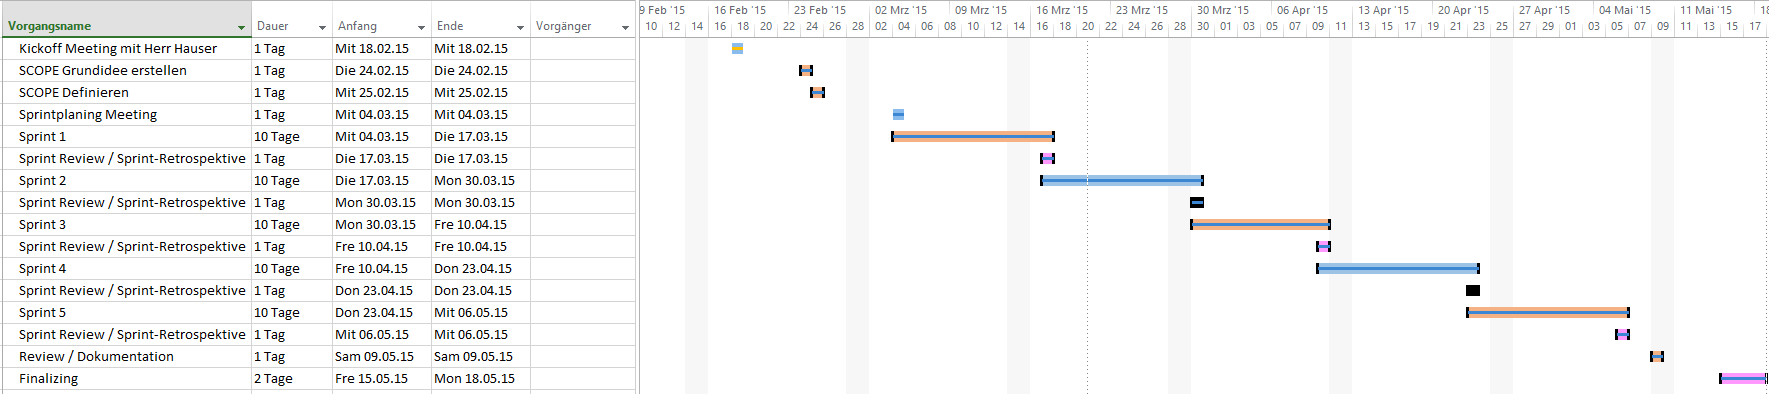
\includegraphics[width=0.8\paperwidth]{PJPlanung}
			\caption{Zeitplanung}
		\end{center}
	\end{figure}	
	
Vielleicht noch was zum Zeitplan sagen ? 
	
\subsection{Product Backlog}
\begin{figure}[h]
		\begin{center}
			\centering
			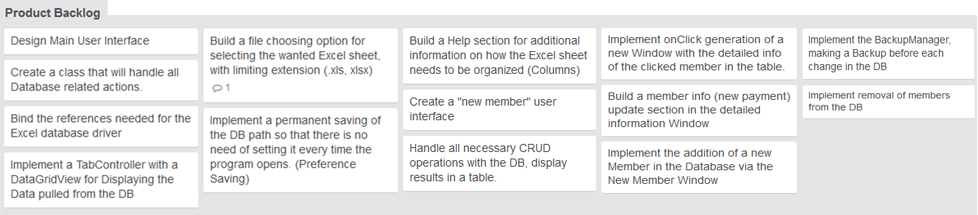
\includegraphics[width=0.8\paperwidth]{ProductBacklog1}
			\caption{Der Produkt Backlog}
		\end{center}
	\end{figure}
	
Lage des Produkt Backlogs noch erklären oder ähnliches.

\subsection{Sprints}
\begin{figure}[h]
	\centering 
	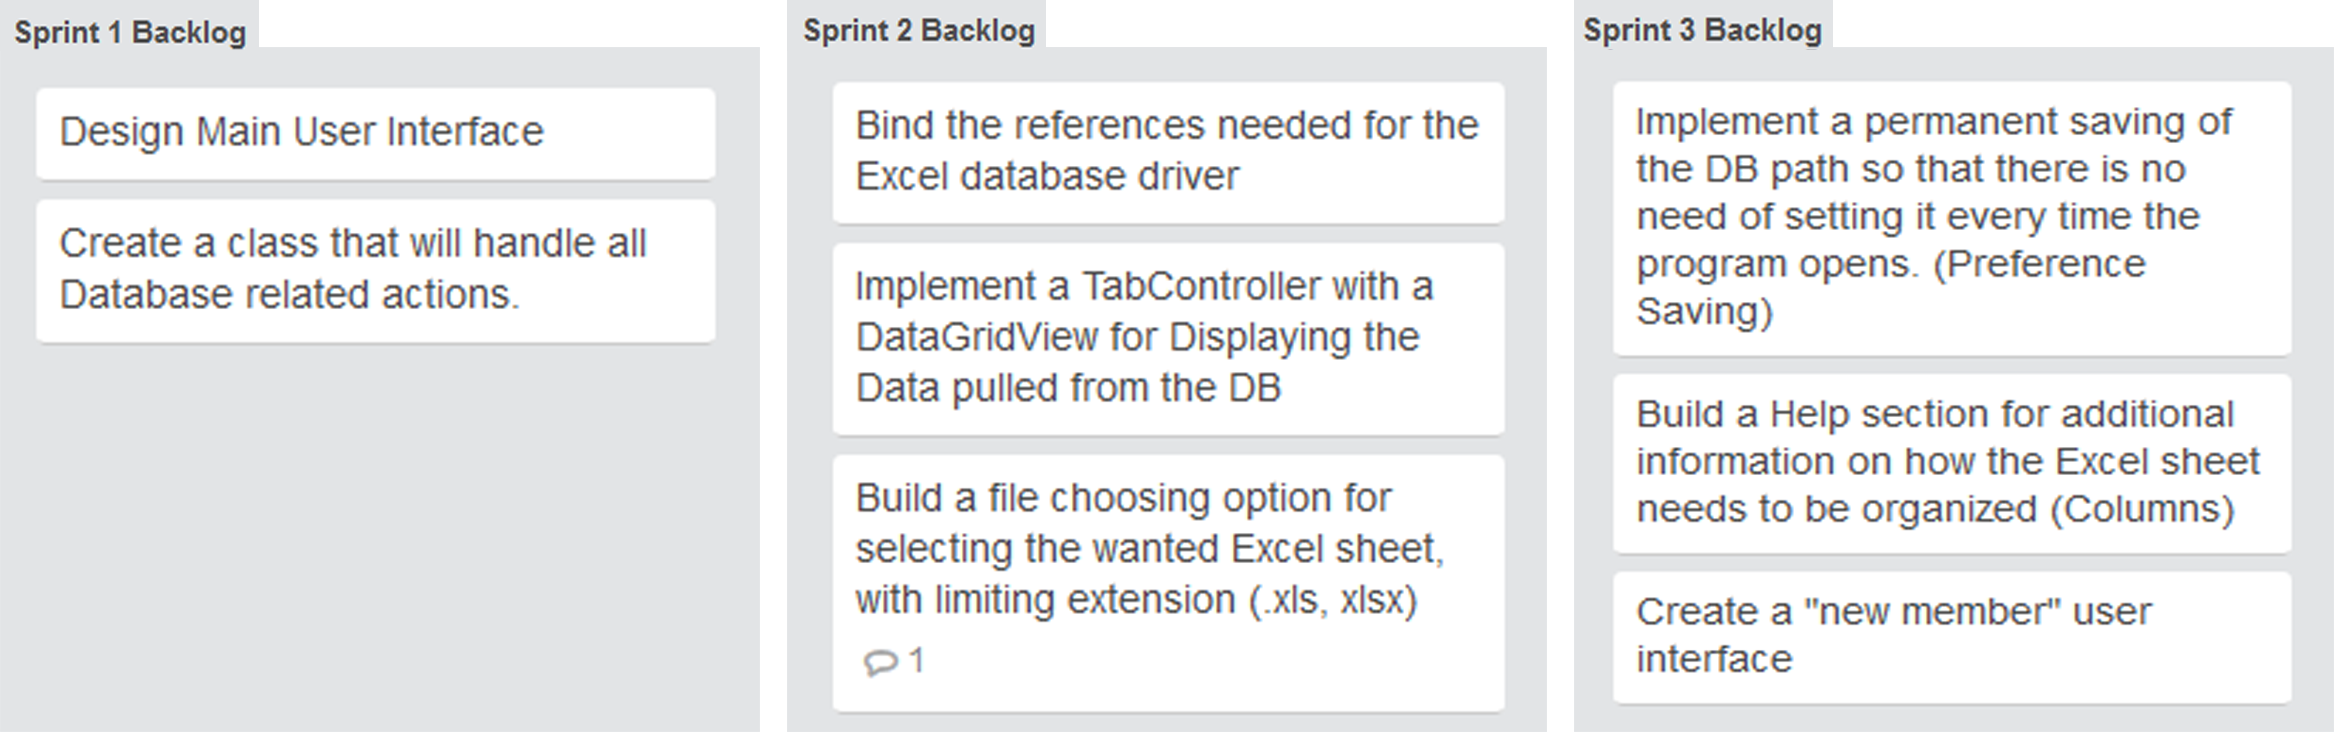
\includegraphics[width=0.6\paperwidth]{Sprint1-3}
	\caption{Sprints 1 - 3}
\end{figure}

\begin{figure}[h]
	\centering
	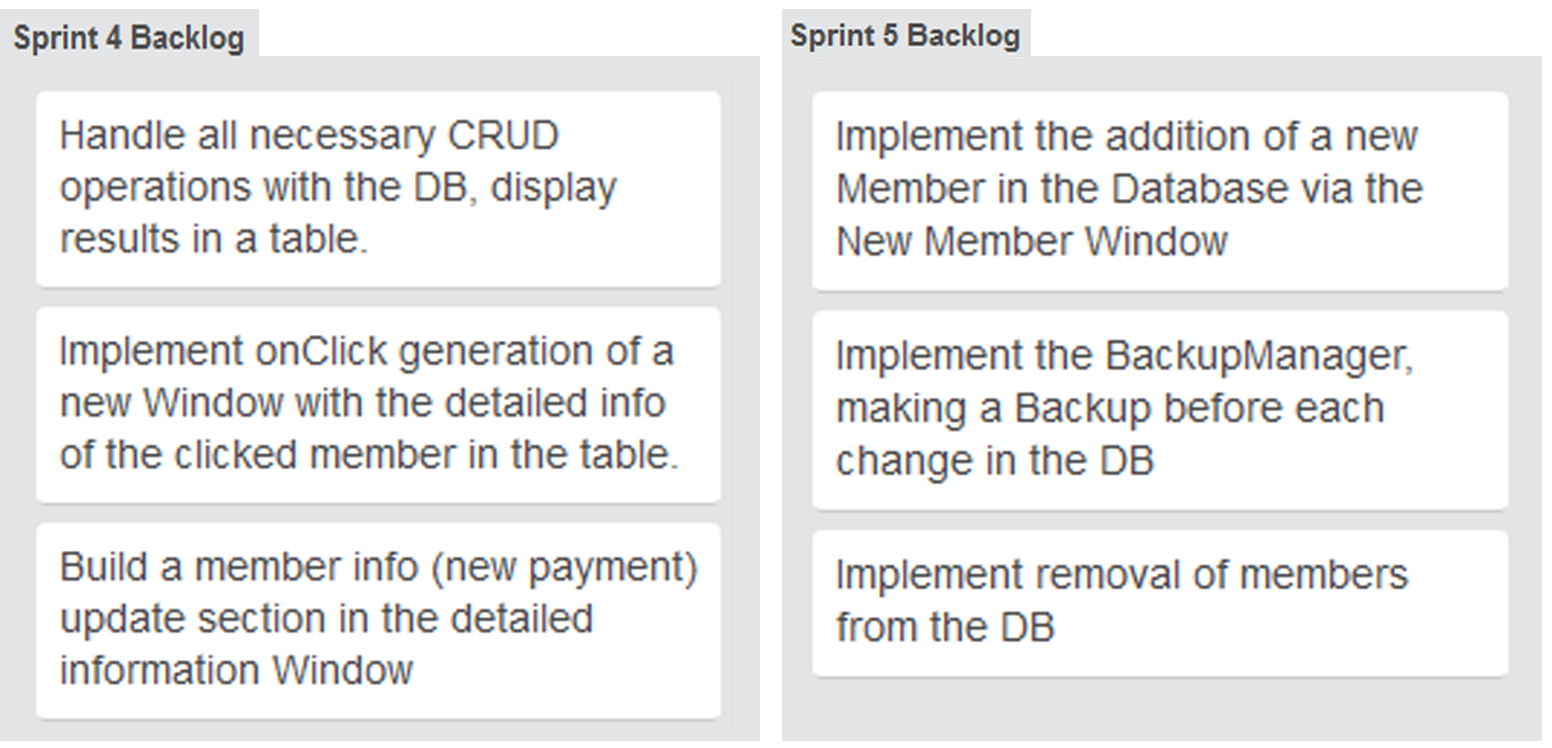
\includegraphics[width=0.4\paperwidth]{Sprint4-5}
	\caption{Sprints 4 - 5}
\end{figure}

\subsection{Sprint Stand-up Meetings}
Protokoll-artig auflisten was wir so besprochen haben usw.

\subsection{Sprint Review}
Review über all die Funktionalitäten und ob wir alles so erledigt haben wie es uns passt.

\newpage

\section{Ablauf der Entwicklung}

\subsection{Modellierung}
Die erste Phase der Entwicklung war das Strukturieren der Software - eine sehr wichtige Phase. Wir wollten ein klares Design von Beginn an, dass uns die Weiterentwicklung ermöglicht.\\
Hier haben wir sehr viel Zeit aufgewendet, mit den Beteiligten sehr viele Szenarien durchgespielt und uns selbst einige Tage Zeit gelassen um über den Funktionsumfang und die Gimmicks eine klare Vorstellung zu erhalten. Die GUI sollte möglichst einfach gehalten sein, was aber nicht heisst, dass sich wenige Funktionen dahinter verbergen. 

\subsubsection{Klassendiagramm}
	
\begin{figure}[h]
	\centering
	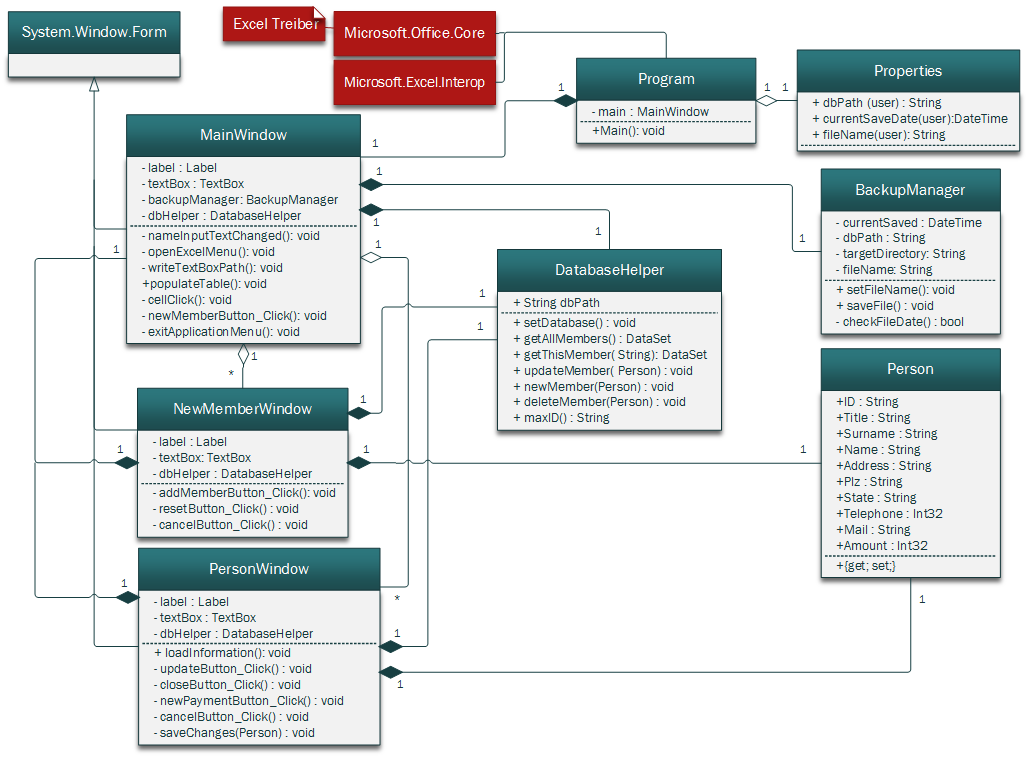
\includegraphics[width=1.05 \textwidth]{KlassendiagrammBild}
	\caption{Klassendiagramm}
\end{figure}

Eintritt in die Applikation geschieht durch die Main() Methode in der Klasse Program. Diese ruft den Konstruktor von MainWindow auf welche die weitere Logik übernimmt. Im Microsoft Visual Studio 2013 werden die GUI Gestaltung und Logik automatisch getrennt, deshalb wurde im Klassendiagramm nur der Logische teil dargestellt.

Die MainWindow Klasse ist das Gehirn der Applikation, es nimmt die Eingaben vom User und leitet sie den entsprechenden Methoden und Klassen weiter. 

Die in Rot dargestellten Referenzen die den OleDB Treiber Beinhalten ermöglichen uns die Verbindung zu Excel Files uns lassen uns diese Auslesen und Beschreiben.


\newpage

\subsubsection{Aktivitäts-Diagramm}
\begin{figure}[h]
	\centering
	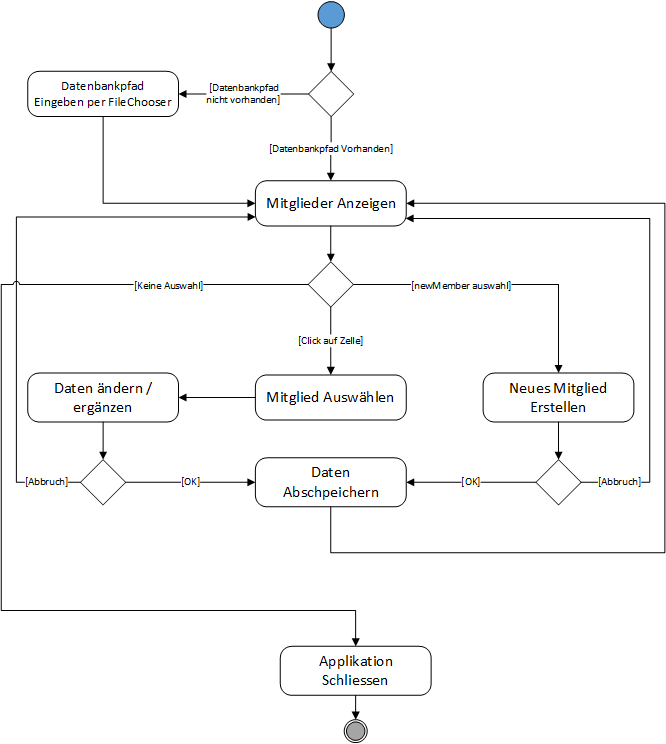
\includegraphics[width=0.8 \textwidth]{Aktivtaetsdiagramm}
	\caption{Aktivitätsdiagramm}
\end{figure}

Hier erkläre ich das was eigentlich dargestellt wurde im Aktivitadosdiagramm.

Lorem ipsum dolor sit amet, consetetur sadipscing elitr, sed diam nonumy eirmod tempor invidunt ut labore et dolore magna aliquyam erat, sed diam voluptua. At vero eos et accusam et justo duo dolores et ea rebum. Stet clita kasd gubergren, no sea takimata sanctus est Lorem ipsum dolor sit amet. Lorem ipsum dolor sit amet, consetetur sadipscing elitr, sed diam nonumy eirmod tempor invidunt ut labore et dolore magna aliquyam erat, sed diam voluptua. At vero eos et accusam et justo duo dolores et ea rebum. Stet clita kasd gubergren, no sea takimata sanctus est Lorem ipsum dolor sit amet.

\newpage

\subsubsection{Sequenzdiagramm}
\begin{figure}[h]
	\centering
	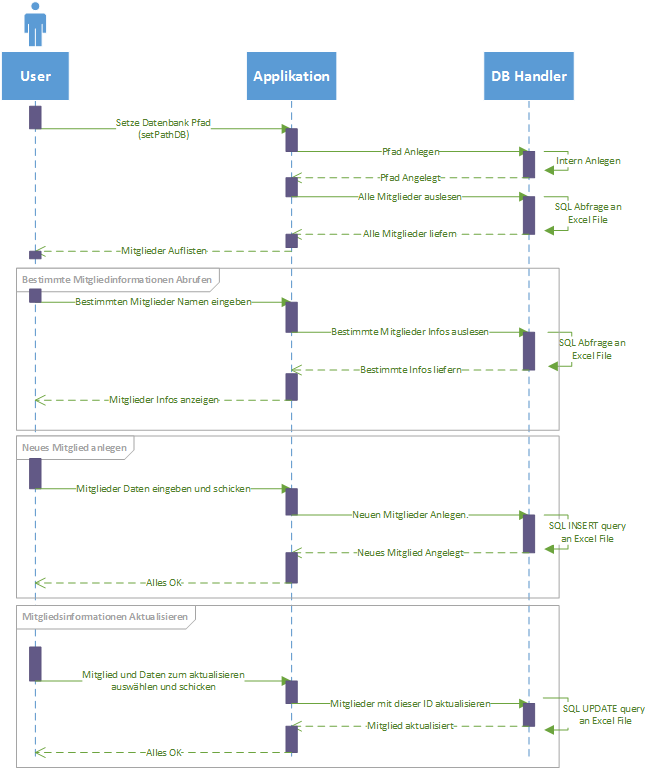
\includegraphics[width=0.8 \textwidth]{Sequenz-Diagramm_v1}
	\caption{Sequenzdiagramm}
\end{figure}

Hier erkläre ich das was eigentlich dargestellt wurde im Sequenzeli.

Lorem ipsum dolor sit amet, consetetur sadipscing elitr, sed diam nonumy eirmod tempor invidunt ut labore et dolore magna aliquyam erat, sed diam voluptua. At vero eos et accusam et justo duo dolores et ea rebum. Stet clita kasd gubergren, no sea takimata sanctus est Lorem ipsum dolor sit amet. Lorem ipsum dolor sit amet, consetetur sadipscing elitr, sed diam nonumy eirmod tempor invidunt ut labore et dolore magna aliquyam erat, sed diam voluptua. At vero eos et accusam et justo duo dolores et ea rebum. Stet clita kasd gubergren, no sea takimata sanctus est Lorem ipsum dolor sit amet.

\newpage


\subsection{GUI}
\subsubsection{Hauptfenster}
\begin{figure}[h]
	\centering
	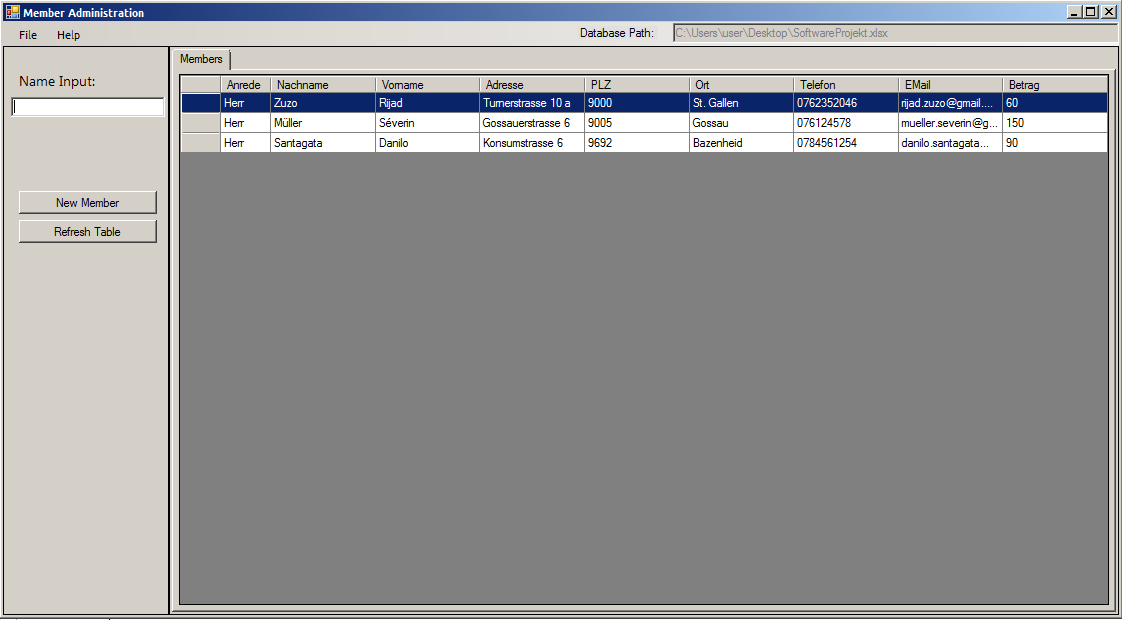
\includegraphics[width=1.0 \textwidth]{MainGUI}
	\caption{Hauptfenster}
\end{figure}
Das GUI wurde so einfach und intuitiv wie möglich gestaltet. Ein einfaches text-input Feld im linken teil lässt den Benutzer schnell den gesuchten Mitglied finden. Ein klick auf den Mitglied in der Tabellenansicht eröffnet ein neues Fenster wie im Bild 7.b) und zeigt alle nötigen Informationen die man auch leicht anpassen kann.


\subsubsection{Aufrufbare Fenster}
 \begin{figure}[h]
 	\centering
 	\begin{subfigure}{.4\textwidth}
 		\centering
 		\includegraphics[width=.5\linewidth]{NewMemberGui}
 		\caption{Neues Mitglied Formular}
 		\label{fig:sub1}
 	\end{subfigure}%
 	\begin{subfigure}{.5\textwidth}
 		\centering
 		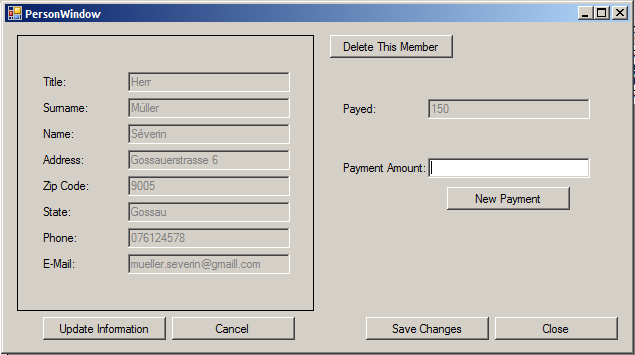
\includegraphics[width=.8\linewidth]{MemberInfoGUI}
 		\caption{Mitgliedsinformation Fenster}
 		\label{fig:sub2}
 	\end{subfigure}
 	\caption{Aufrufbare Fenster}
 	\label{fig:test}
 \end{figure}
 
\subsection{Database Handling}
Schwierigkeiten bei den Referenzen, Voraussetzungen zur Verbindung usw.

\subsection{Backup Management}
Ansätze für ein effizientes Backuping :).

\subsection{Stunden Journal}

\section{Testen}
Wie beim Testen vorgegangen wurde!

\newpage

\section{Ziel}
\subsection{Resultat}
\subsection{Gelerntes}

\end{document}